\section{Boolean Encoding over $\Z_p$ and Homomorphic Evaluation Strategy Between $\B$ and $\Z_p$}
\label{sec:homorphic_layer}

To evaluate Boolean functions in TFHE, one could use the vanilla TFHE with $p=2$. The problem is that the only evaluable function would be the \texttt{XOR} operation. To evaluate the other operators, the solution of \cite{cryptoeprint:2018/421} which is also implemented in the \texttt{tfhe-rs} library \cite{tfhe-rs} is to take a larger $p$, specifically $p=8$. This allows all the operations of the Boolean algebra to be carried out, however the negacyclicity problem introduced in Section \ref{sec:bootstrapping} arises because $8$ is even. Their solution to this issue is to keep a \emph{bit of padding} fixed to zero, i.e., the values in $\Z_p$ have their most significant bit fixed to zero. This restriction has a heavy impact on performances, because it requires a bootstrapping after each Boolean gate to make sure no data ever overflows in the most significant bit.

Our solution makes use of \emph{odd} values for $p$, which allows us to remove this constraint of padding and to perform more operations without bootstrapping. To do so, we had to slightly adapt the bootstrapping procedure of TFHE to support odd moduli. We explain this tweak in Section  \ref{sec:TFHE_adaptation}.

Moreover, the PBS described in Section \ref{sec:bootstrapping} takes only one input and so can only evaluate univariate functions. The common solution to evaluate multivariate functions is to concatenate several input ciphertexts into one by shifting the MSB of each input and to sum them all. The problem is that the number of message bits cannot grow too much because the other parameters of the \LWE problem must grow accordingly, degrading the performances. As a consequence, the performances quickly degrades as the arity of the function increases. Our approach consists in removing the padding bit and using a combination of homomorphic additions before a PBS to evaluate a function for \emph{any} number of inputs with the cost of a single PBS.


To this purpose, we propose a construction in which we embed Boolean values in $\Z_p$ for well-chosen values of $p$, forming an ``intermediate homomorphic layer'' between $\B$ and $\Z_q$. In the following, we explain how we define such a layer, and we describe our new strategy to evaluate Boolean functions in a more efficient way without considering the circuit representation of the function.


\subsection{Encoding of $\B$ over $\Z_p$}

To represent Boolean values over $\Z_p$, we use a mapping function that we call a \emph{$p$-encoding}:

\begin{definition}[$p$-encoding]
    A \emph{$p$-encoding} is a function $\Encoding: \mathbb B \mapsto 2^{\mathbb Z_p}$ that maps the Boolean space to a subset of the discretized torus. A $p$-encoding is \emph{valid} if and only if:
    \begin{equation}
        \begin{cases}
            \Encoding(0) \cap \Encoding(1) = \emptyset~\text{ and}\\
            \text{if $p$ is even:} ~\forall \:x \in \mathbb Z_p, \forall \:b \in \B: x \in \Encoding(b) \iff \left [ x + \frac p 2 \right ]_p \notin \Encoding(b)
        \end{cases}
    \label{def:validity}
    \end{equation}
    We call this last property \emph{relaxed negacyclicity}.
    \label{def:encoding}
\end{definition}


\begin{figure}
  \centering
    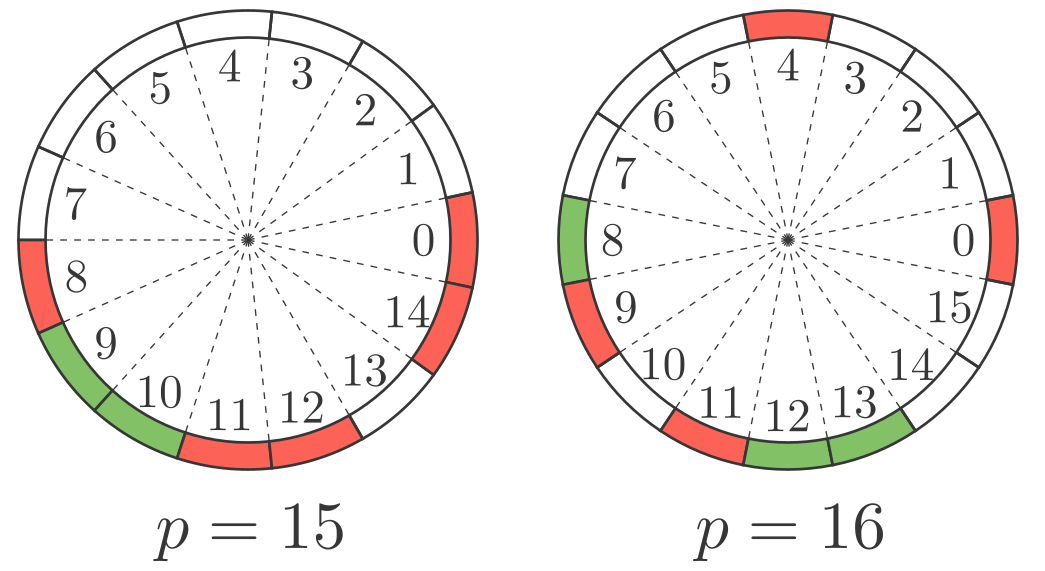
\includegraphics[scale=0.2]{images/encoding_example_double.png}

  \caption{Representation of two valid $p$-encodings. The green part represents $\Encoding(1)$,  and the red part $\Encoding(0)$. Note that the relaxed negacyclity is respected by the $p$-encoding on the right-hand figure as $p$ is even.}
  \label{fig:encodings}
\end{figure}


In our approach when we need to encrypt a bit, we apply a $p$-encoding to embed it on $\Z_p$, then we encrypt the result using the classical setup of TFHE.  When new values are freshly encrypted or produced by a PBS, only one element of $ \Z_p$ is chosen for each bit. We call such an encoding a canonical $p$-encoding:

\begin{definition}[Canonical Encoding]
    A $p$-encoding $\Encoding$ is said \emph{canonical} if and only if it is valid and $\left| \Encoding(0) \right| = \left| \Encoding(1) \right| = 1$
    \label{def:canonical}
\end{definition}


Let $c$ be a ciphertext encoding a bit $b$ under a $p$-encoding $\Encoding$, where $\Encoding$ is an arbitrary valid encoding: its associated subsets can be any subset of $\Z_p$ as long as the validity requirements of (\ref{def:validity}) are fulfilled. One can transform the ciphertext $c$ into another ciphertext $c'$ encoded under any \emph{canonical} $p$-encoding, possibly under a different $p$, by simply performing a PBS.


\begin{property} [Reduction to a canonical encoding]
    \label{prop:cast_valid_to_canonical}
    Let $\Encoding$ be a valid $p$-encoding and $\Encoding'$ a canonical $p'$-encoding. We denote $\alpha' = \Encoding'(0)$ and $\beta' = \Encoding'(1)$. Let $c$ be a ciphertext encrypting a bit $b$ under $\Encoding$. Then, one can produce a ciphertext $c'$ encrypting the same bit $b$ under $\Encoding'$ by applying a PBS on $c$. This PBS performs the function :
    \[
        \begin{aligned}
            \texttt{Cast}_{\Encoding \mapsto \Encoding'}~:~& \Z_p \mapsto \Z_{p'}\\
            & x \mapsto \begin{cases}
                            \alpha' & \text{ if } x \in \Encoding(0)\\
                            \beta' & \text{ if } x \in \Encoding(1)\\
                            \bot & \text{ otherwise.}
                        \end{cases}
        \end{aligned}
    \]
    Here, $\bot$ simply denotes a placeholder value for a state that cannot be reached.
\end{property}



Our goal is to represent the Boolean function we want to evaluate with a sum of $p$-encodings (we define what we mean by ``sum of $p$-encoding'' in Section \ref{sec:new_strategy}).  When sums are carried out on ciphertexts (and so homomorphically on the underlying $p$-encodings), the sets $\Encoding(0)$ and $\Encoding(1)$ of the $p$-encodings may move, grow, shrink, but they should never overlap as it would result in a loss of information. As we removed the need of a bit of padding, we do not need to track a potential overflow of data (informally we say that ciphertexts are free to ``go around the torus''). After the sum, the encoding of the result can be reset to a canonical one with a PBS to allow further computation. Or, if the homomorphic computation is over, the result can be recovered by decrypting the ciphertext and checking in which partition the decrypted value lies.


The next subsection explains in further details the process of evaluating Boolean functions on with $p$-encodings.



\subsection{A New Strategy for Homomorphic Boolean Evaluation}
\label{sec:new_strategy}



In the following, we consider two Boolean variables $x$ and $y$ and their two respective encodings over $\Z_p$: 
\begin{equation}
\Encoding_x = 
\EncDef{\{\alpha_i\}_{0 \le i \le l_0}}{\{\beta_i\}_{0 \le i \le l_1}} \text{ and } \Encoding_y = \EncDef{\{\alpha'_i\}_{0 \le i \le l'_0}}{\{\beta'_i\}_{0 \le i \le l'_1}}
\label{eq:encoding_definition}
\end{equation}


Let $f$ be a bivariate Boolean function and let us construct two sets $\mathcal{P}_0$ and $\mathcal{P}_1$ such that:
\begin{equation}
    \mathcal{P}_b = \{[\gamma + \delta]_p \mid (\gamma, \delta) \in \Encoding_x(b_x) \times \Encoding_y(b_y) \text{ and } f(b_x, b_y) = b \text{ with } (b_x, b_y) \in \B^2\}~\forall~b \in \B.
    \label{def:sets_p}
\end{equation}

We say that the sum of $p$-encodings $\Encoding_x + \Encoding_y$ is \emph{suitable for the evaluation of $f$} if and only if $\mathcal{P}_0 \cap \mathcal{P}_1 = \emptyset$. The definition can be generalized to any number of arguments $\ell$ for $f$. For a given $f$, finding such correct encodings is not trivial. We elaborate further on this point in Section \ref{sec:search}. 

If $\Encoding_x$ and $\Encoding_y$ are suitable for $f$, then one can use the computed sets $\mathcal{P}_b$ to construct a new $p$-encoding \[\Encoding_z = \EncDef{\mathcal{P}_0}{\mathcal{P}_1}\] that encodes the bit $f(x, y)$. As $\Encoding_z$ is valid, then the clear value of the bit can be recovered by decryption, or further computations can be performed without the need of a bootstrapping. 


\begin{definition}[Application of a function to a vector of encodings]
    Let $f:\B^\ell \mapsto \B$ be a Boolean function and let $\Encoding = (\Encoding_1, \dots, \Encoding_l)$ be a vector of $p$-encodings. We define $f(\Encoding)$ by:
    \[f(\Encoding) = \EncDef{\mathcal{P}_0}{\mathcal{P}_1}\]
    with: 
    \[\mathcal{P}_b = \left \{ \left [ \sum_{i=1}^{l} \gamma_i \right ]_p \mid (\gamma_1, \dots, \gamma_l) \in \prod_{i=1}^\ell \Encoding_i(b_i) \text{ and } f(b_1, \dots, b_l) = b \right \} \forall b \in \B\]

We stress that $f(\Encoding)$ is a valid $p$-encoding if and only of $\mathcal{P}_0 \cap \mathcal{P}_1 = \emptyset$.
\end{definition}


Let us illustrate the latter definition on two toy example. We consider the two Boolean operators $\&$ and $\oplus$. The $p$-encoding resulting of the function $f: (x, y) \mapsto x ~\&~ y$ is: 

\begin{equation}
\Encoding_\& = \begin{cases}
0 \mapsto \{\alpha_i + \alpha'_j\}_{\substack{0\le i \le l_0 \\ 0 \le j \le l_0'}} \cup \{\alpha_i + \beta'_j\}_{\substack{0 \le i \le l_0 \\ 0 \le j \le l'_1}} \cup \{\alpha'_i + \beta_j\}_{\substack{0 \le i \le l'_0 \\ 0 \le j \le l_1}}\\
1 \mapsto \{\beta_i + \beta'_j\}_{\substack{0\le i \le l_1 \\ 0 \le j \le l_1'}}
\end{cases}
\label{eq:encoding_and}
\end{equation}
and the $p$-encoding resulting of the operation $f: (x, y) \mapsto x \oplus y$ is:

\begin{equation}
\Encoding_\oplus = \begin{cases}
0 \mapsto \{\alpha_i + \alpha'_j\}_{\substack{0\le i \le l_0 \\ 0 \le j \le l_0'}} \cup \{\beta_i + \beta'_j\}_{\substack{0 \le i \le l'_0 \\ 0 \le j \le l'_1}}\\
1 \mapsto \{\alpha_i + \beta'_j\}_{\substack{0\le i \le l_0 \\ 0 \le j \le l_1'}} \cup \{\alpha'_i + \beta_j\}_{\substack{0\le i \le l_0' \\ 0 \le j \le l_1}} \\
\end{cases}
\label{eq:encoding_xor}
\end{equation}
%
Figure \ref{fig:operations} further illustrates this construction for these two operations.

\begin{figure}
    \centering
    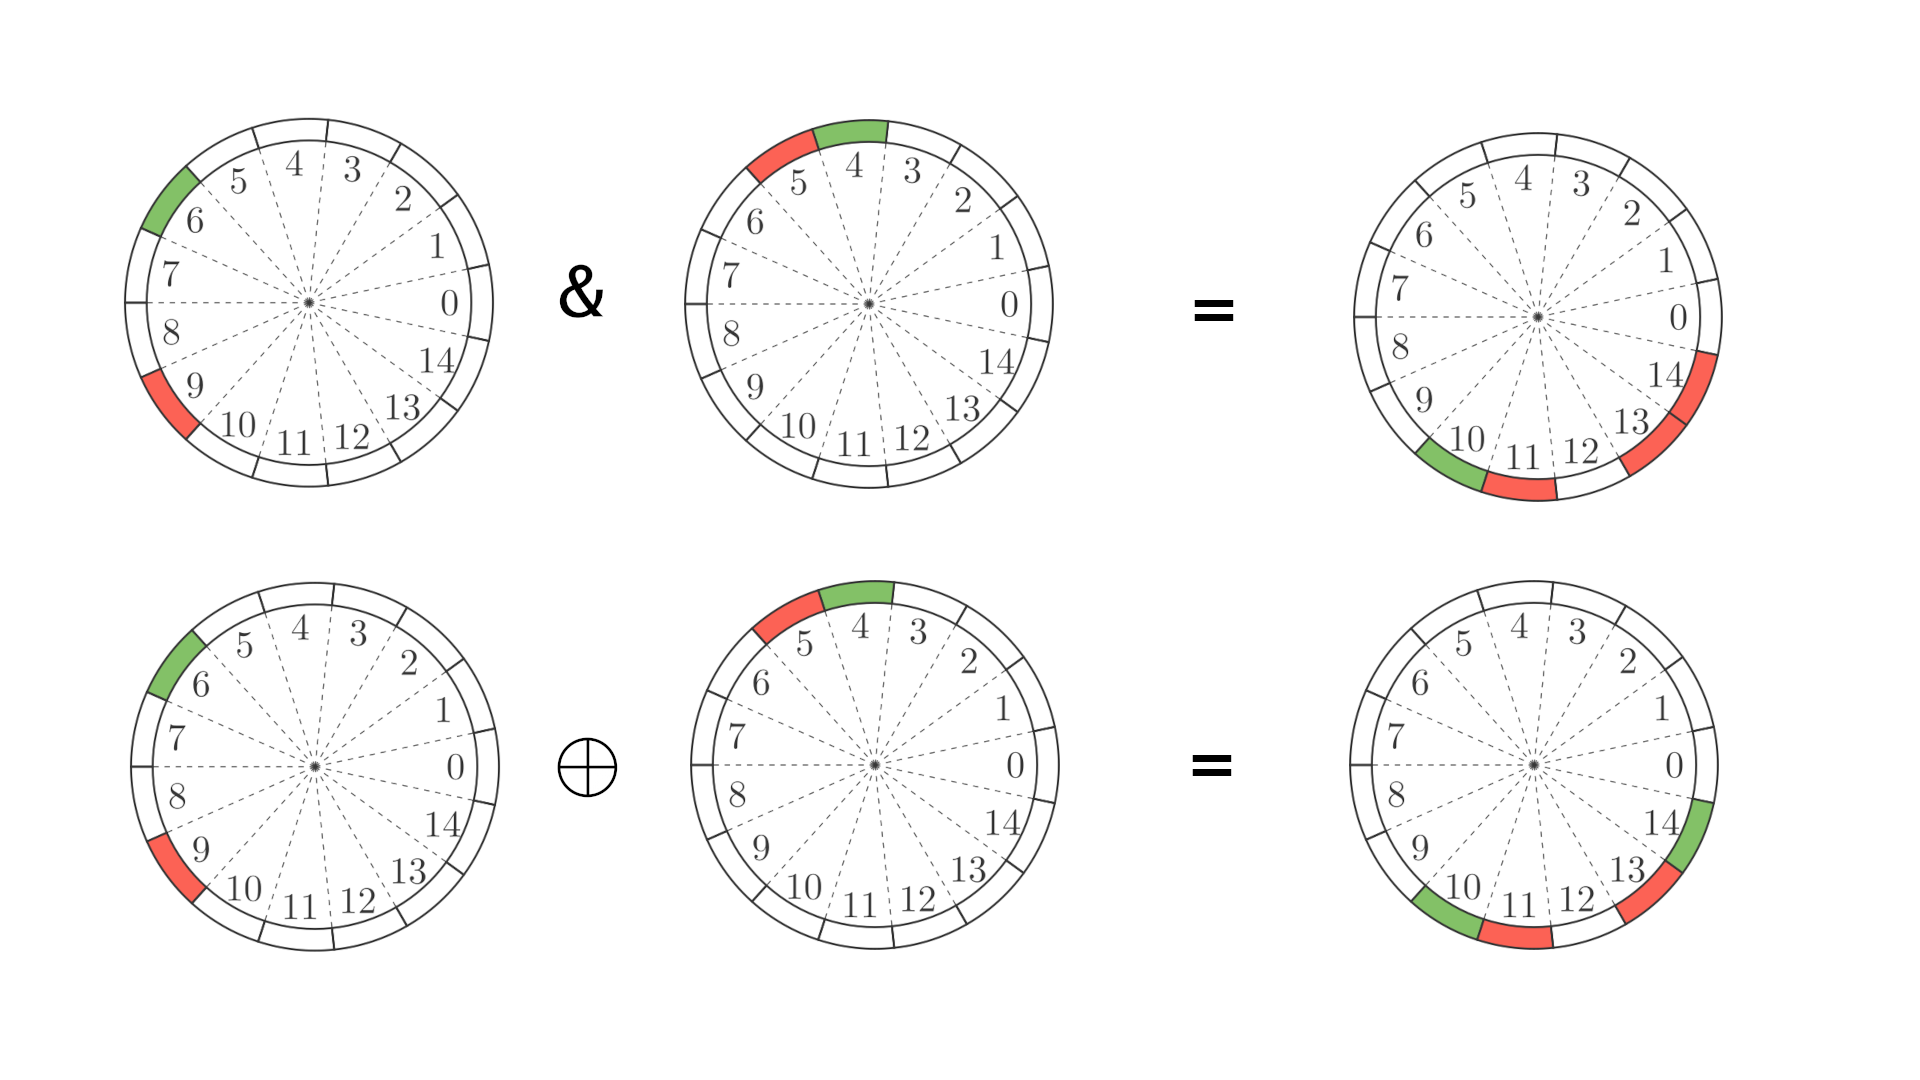
\includegraphics[width=\textwidth]{images/operators.png}
    \caption{Starting from two canonical encodings, we produce two new $p$-encodings corresponding to the results of the $\&$ and the $\oplus$ operations.}
    \label{fig:operations}
\end{figure}


To wrap up, here is our proposed framework to evaluate a Boolean function $f: \B^\ell \mapsto \B$ given a vector of suitable $p$-encodings $\Encoding = (\Encoding_1, \dots, \Encoding_l)$:

\begin{enumerate}
\item Encrypt each input $b_i$ with some canonical $p$-encoding $\Encoding_i$ into a ciphertext $c_i$ such that $\Encoding_{sum} = f(\Encoding_1, \dots, \Encoding_\ell)$ is a valid encoding.
\item For a Boolean function $f$ to be evaluated on $b_1, \dots, b_l$, compute homomorphically the sum of the ciphertexts $c = c_1 + \dots + c_l$. This yields an encryption of $b = f(b_1, \dots, b_l)$, encoded with a valid $p$-encoding $\Encoding_{sum} = f(\Encoding_1, \dots, \Encoding_l)$.
\item \begin{enumerate}
    \item If the result is directly required by the client, $c$ is returned as ciphertext which can be decrypted to get the result in $\Z_p$ and associated to the right Boolean value.
    \item If the result is reused in further homomorphic computations, a PBS calculating $\texttt{Cast}_{\Encoding_{sum} \mapsto \Encoding_{new}}$ on the result is computed (like introduced in Property \ref{prop:cast_valid_to_canonical}), with $\Encoding_{new}$ a new canonical $p$-encoding. The resulting value can then be used as an input for a next Boolean function.
    \end{enumerate}
\end{enumerate}

Let us formalize this process by defining the notion of \textit{gadget associated to a Boolean function $f$} :
\begin{definition}[Gadget]
    Let $f$ be a Boolean function of arity $\ell$.
    A gadget associated to $f$ is an homomorphic operator defined by a tuple $\Gamma = \left ( \vec{\Encoding_{in}} = (\Encoding_{in}^{(1)}, \dots, \Encoding_{in}^{(\ell)}), \Encoding_{out}, p_{in}, p_{out} \right )$ such that:
    \begin{itemize}
        \item All the elements of $\vec{\Encoding_{in}}$ are $p_{in}$-encodings, and $\Encoding_{out}$ is a canonical $p_{out}$-encoding.
        \item The encoding $\Encoding_{sum} = f(\Encoding_{in}^{(1)}, \dots, \Encoding_{in}^{(\ell)})$ is a valid encoding.
    \end{itemize}
Applying a gadget to ciphertexts  $c1, \dots, c_\ell$, that encrypt the bits $b_1, \dots, b_\ell$, produces a new ciphertext $c'$ encrypting the bit $f(b_1, \dots, b_\ell)$ under the $p_{out}$-encoding $\Encoding_{out}$. To do so, we perform the following algorithm:
\begin{itemize}
    \item Constructing an intermediate ciphertext $c_{inter} = \sum_{i=1}^{\ell} c_i$ using the homomorphic sum of TFHE. This ciphertext encrypts $f(b_1, \dots, b_\ell)$ under the $p_{in}$-encoding $f(\Encoding_1, \dots, \Encoding_\ell)$.
    \item Reducing the encoding of $c_{inter}$ from $\Encoding_{inter}$ to $\Encoding_{out}$ by applying a PBS on $c_{inter}$ performing the function $\texttt{Cast}_{\Encoding_{inter} \mapsto \Encoding_{out}}$. This produces the expected result $c'$.
    \end{itemize}
\label{def:gadget}
\end{definition}


The advantage of this construction is that only one PBS is performed to apply the function. Moreover, depending on the function, the input size of the PBS lookup table might be much smaller than the arity of the function. Gadgets can be seen as a way to compress several Boolean operators into a single evaluation of univariate look-up table.
Of course, for a given $p_{in}$ and a given $f$, such a gadget may not exist. In such a case, two solutions can be considered:
\begin{itemize}
    \item Increasing the value of $p_{in}$ (e.g.  taking $p_{in} \ge 2^\ell$ always works, but is very inefficient).
    \item Splitting the function into a graph of subfunctions, and evaluating each one with a gadget.
\end{itemize}

The question of constructing valid gadgets for a given $f$ is treated in Section \ref{sec:search}. The question of efficiently splitting a function is treated in Section \ref{sec:graphs}.


\paragraph{Example:} We illustrate our approach with a simple working example: let $f$ be a basic multiplexing function, such that  $$
f(a, b, c) = \begin{cases}
    a \text{ if } c = 1\\
    b \text{ if } c = 0
\end{cases}
$$
Instead of leveraging its Boolean representation $f(a, b, c) = a \& c \oplus b \& \Bar{c}$, which would cost 3 PBS with the approach of \cite{cryptoeprint:2018/421}, our strategy consists in constructing a gadget and apply it to the inputs $a$, $b$ and $c$, which takes only one PBS. Here is the step-by-step procedure:

\begin{enumerate}
    \item Encrypting the bits with the $7$-encodings:\[\Encoding_a = \Encoding_b = \EncDefOne{1} \text{ and } \Encoding_c = \EncDefOne{2}\].
    \item Applying the function $f$ on the $7$-encodings by summing the ciphertexts, producing a valid $7$-encoding:\[\Encoding_{sum} = \EncDef{\{0, 1, 2, 5\}}{\{3, 4, 6\}}\] At this point, only sums have been performed on the ciphertexts.
    \smallskip
    \item With one PBS, resetting the result to a target canonical $p$-encoding (with any $p$), for example \[\Encoding_{new} = \EncDefOne{1} \text{ with } p=7\]
\end{enumerate}

A visualization of this procedure can be found in Figure \ref{fig:illustration}. We just defined the gadget $\Gamma = \left ( (\Encoding_a, \Encoding_b, \Encoding_c), \Encoding_{new}, 7, 7\right )$.

\begin{figure}
    \centering
    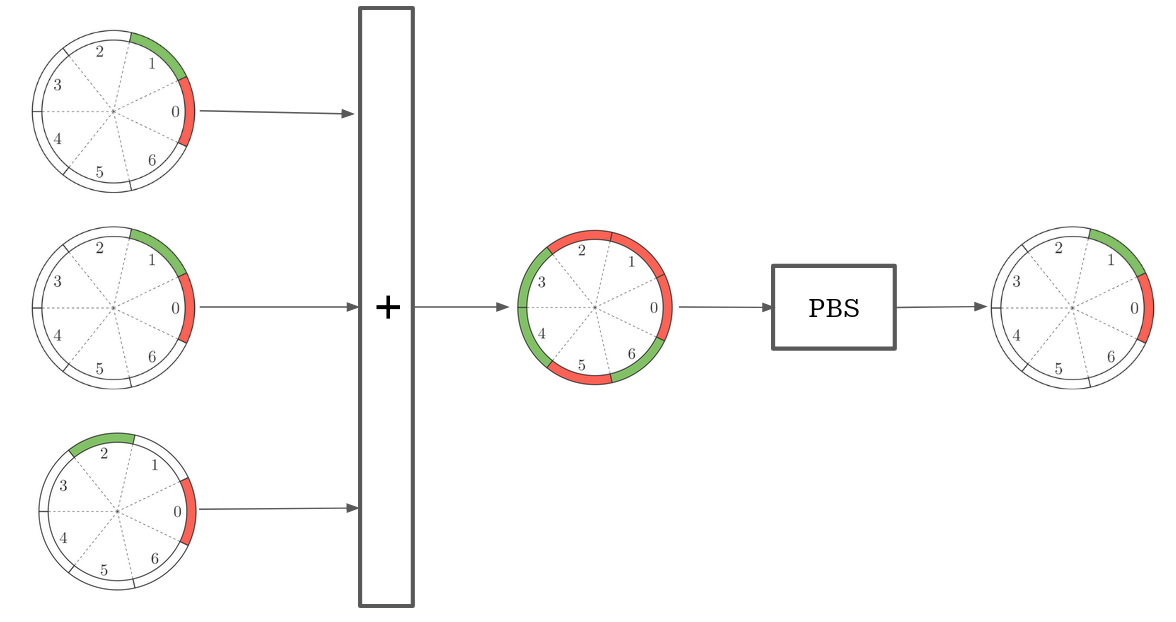
\includegraphics[width=\linewidth]{images/illustration_framework.png}
    \caption{Illustration of an execution of the framework for the multiplexing function.}
    \label{fig:illustration}
\end{figure}


\subsection{Encoding Switching}
\label{encoding_switching}

To apply a gadget to a given ciphertext, it has to be encrypted under the right encoding. Thus, we need a method to homomorphically switch the encoding of a ciphertext. This allows as well to plug the output of any gadget on the input of any other one, and so to evaluate a chain of gadgets as long as we want. In the following, we explore different possibilities of encoding switching. Let us begin with some trivial cases:

\begin{property}[Encoding switching with a sum by a constant]
    \label{prop:sum_constant}
    Let $x$ be a ciphertext encoded under $\Encoding_x = \EncDef{\{\alpha_i\}_{0 \le i \le l_0}}{\{\beta_i\}_{0 \le i \le l_1}} $ and $a \in \Z_p$ a constant. The encoding of $x$ can be switched to:
    \[\Encoding_x' = \EncDef{\{\modulo{\alpha_i + a}{p}\}_{0 \le i \le l_0}}{\{\modulo{\beta_i + a}{p}\}_{0 \le i \le l_1}}\] by an homomorphic addition of the ciphertext $x$ and the clear value $a$. 
\end{property}

\begin{proof}
    All the elements of $\Encoding_x'(0)$ (resp. $\Encoding_x'(1)$) are offset by exactly $a$ from their counterparts in $\Encoding_x(0)$ (resp. $\Encoding(1)$). Thus, if the original encoding $\Encoding_x$ was valid, then $\Encoding_x(0) \cap \Encoding_x(1) = \emptyset$. So we trivially get  $\Encoding_x'(0) \cap \Encoding_x'(1) = \emptyset$ and thus the validity of $\Encoding_x'$.
\end{proof}


\begin{property}[Encoding switching with multiplication by a constant]
    \label{prop:mult_constant}
    Let $x$ be a ciphertext encoded under $\Encoding_x = \EncDef{\{\alpha_i\}_{0 \le i \le l_0}}{\{\beta_i\}_{0 \le i \le l_1}} $ and $a \in \Z_p$ a constant value prime with $p$. The encoding of $x$ can be switched to:
    \[\Encoding'_x = \EncDef{\{[a \cdot \alpha_i]_p\}_{0 \le i \le l_0}}{\{[a \cdot \beta_i]_p\}_{0 \le i \le l_1}}\]
    by an homomorphic multiplication of the ciphertext $x$ by the clear value $a$.
\end{property}
\begin{proof}
As $a$ is prime with $p$, the multiplication by $a$ is a bijection from $\Z_p$ to $\Z_p$. By definition, all the $\alpha_i$'s are different of the $\beta_i$'s. If we apply a bijection on them, the inequalities are conserved.
\end{proof}

Note that the condition of primality between $a$ and $p$ is a sufficient condition for the multiplication to be a valid encoding switching, but is not necessary. In particular, one other case is particularly useful in practice:

\begin{property}[Encoding switching for a canonical encoding containing a zero]
\label{prop:mult_from_1}
    Let $x$ be a ciphertext encoded under the $p$-encoding: $\Encoding_x = \EncDefOne{1}$ and let $a \in \Z_p \setminus \{0\}$. Then, it can be switched to: $\Encoding'_x = \EncDefOne{a}$ by a simple homomorphic multiplication between the ciphertext $x$ and the clear value $a$.
    This holds as well if $\Encoding(0)$ and $\Encoding(1)$ swapped.
\end{property}

\begin{proof}
    The property is trivial by the linear homomorphism of the TFHE scheme.
\end{proof} 

These techniques are powerful because they do not require any bootstrapping, so they can be considered as free in terms of performances. However, any valid $p$-encoding can be turned into any other one with a programmable bootstrapping, even with a different modulus $p$. A reduced version of this is given by Property \ref{prop:cast_valid_to_canonical}, but it can be extended to any valid output $p$-encoding.

\begin{property} [Arbitrary encoding switching with a PBS]
    Let $c$ be a ciphertext encoded under $\Encoding$. Its encoding can be switched to $\Encoding'$ (even with a different modulus $p'$) by applying a PBS on $c$ evaluating the function     \begin{align}
        \texttt{Cast}_{\Encoding \mapsto \Encoding'}~:~& \Z_p \mapsto \Z_{p'}\\
        & x \mapsto \begin{cases}
                        \alpha' \in \Encoding'(0) & \text{ if } x \in \Encoding(0)\\
                        \beta' \in \Encoding'(1) & \text{ if } x \in \Encoding(1)\\
                        \bot & \text{ otherwise.}
                    \end{cases}
    \end{align}
    Here, $\bot$ simply denotes an arbitrary placeholder value, as it will never be reached.
    \label{prop:enc_switch_pbs}
\end{property} 




 See Sections \ref{sec:bootstrapping} and \ref{sec:accumulator} for a more in-depth insight on the actual procedure of programmable bootstrapping.
